\RequirePackage{currfile} 
\documentclass{beamer}



%%%%%%%%%%%%%% PACKAGES %%%%%%%%%%%%%%%%%%%%%
\usepackage{textpos}   
\usepackage{graphicx} % Allows including images
\usepackage{booktabs} % Allows the use of \toprule, \midrule and \bottomrule in tables
%\usepackage{biblatex} % Allows for \cite 
\usepackage[utf8]{inputenc}
\usepackage{tikz} \usetikzlibrary{calc, arrows.meta, intersections, patterns, positioning, shapes.misc, fadings, through,decorations.pathreplacing}
\usepackage[usenames,dvipsnames]{xcolor}
\usepackage{colortbl}
\usepackage{multicol}
\usepackage{multirow}
\usepackage{caption}
%\usepackage{block} %blocks for statements
\usepackage{comment}
\usepackage[round,authoryear]{natbib}
\usepackage[absolute,overlay]{textpos}
\usepackage{array} %To hide columns
\usepackage{stix} % For arrows
\usepackage{forest}

\usepackage{array} % To hide columns
\newcolumntype{H}{>{\setbox0=\hbox\bgroup}c<{\egroup}@{}}

\forestset{qtree/.style={for tree={parent anchor=south, 
           child anchor=north,align=center,inner sep=0pt}}}



% Custom block colors for better appearance
\setbeamercolor{block title}{bg=blue!20,fg=black}
\setbeamercolor{block body}{bg=blue!10,fg=black}
\setbeamertemplate{blocks}[rounded][shadow=true]

%To edit bullet point sizes
\setbeamertemplate{itemize item}{\textbullet}
\setbeamertemplate{itemize subitem}{\raisebox{0.25ex}{\scalebox{0.6}{\textbullet}}}

% To have numbering
\setbeamertemplate{footline}{
    \hfill\insertframenumber\hspace{1em}\vspace{1em}
}




\definecolor{ColorOne}{named}{MidnightBlue}
\definecolor{ColorTwo}{named}{Dandelion}
\definecolor{ColorThree}{named}{Plum}

\tikzstyle{descript} = [text = black,align=center, minimum height=1.8cm, align=center, outer sep=0pt,font = \footnotesize]
\tikzstyle{activity} =[align=center,outer sep=1pt]

%% Change the bg color to adjust your transition slide background color!
\definecolor{sagegreen}{RGB}{185,205,190} 
\newenvironment{transitionframe}{
  \setbeamercolor{background canvas}{bg=sagegreen}
  \begin{frame}}{
    \end{frame}
}




%%%%%%%%%%%%%% COMMANDS %%%%%%%%%%%%%%%%%%%%%
\newcommand{\progressbar}{%
\pgfmathsetmacro{\theta}{360/\inserttotalframenumber*\insertframenumber}
\begin{tikzpicture}[scale=0.025]
\fill[blue] (0,0) circle (9);
\fill[green] (0,0) -- (9,0) arc (0:-\theta:9);
\fill[white] (0,0) circle (5);
\node at (0,0) {\insertframenumber};
\end{tikzpicture}
}

%%% TIKZ STUFF
\tikzset{   
        every picture/.style={remember picture,baseline},
        every node/.style={anchor=base,align=center,outer sep=1.5pt},
        every path/.style={thick},
        }
\newcommand\marktopleft[1]{%
    \tikz[overlay,remember picture] 
        \node (marker-#1-a) at (-.3em,.3em) {};%
}
\newcommand\markbottomright[2]{%
    \tikz[overlay,remember picture] 
        \node (marker-#1-b) at (0em,0em) {};%
}
\tikzstyle{every picture}+=[remember picture] 
\tikzstyle{mybox} =[draw=black, very thick, rectangle, inner sep=10pt, inner ysep=20pt]
\tikzstyle{fancytitle} =[draw=black,fill=red, text=white]
%%%% END TIKZ STUFF

% Custom commands for colored citations
\newcommand{\citered}[1]{{\color{red}\cite{#1}}}
\newcommand{\citeblue}[1]{{\color{blue}\cite{#1}}}
\newcommand{\citesmall}[1]{{\footnotesize\cite{#1}}}
\newcommand{\citetiny}[1]{{\tiny\cite{#1}}}

% Commands for highlighting overlays
\newcommand{\highlightbox}[5]{% x, y, width, height, color
    \tikz[overlay,remember picture]{
        \draw[#5, ultra thick, rounded corners] 
        ([shift={(#1,#2)}]current page.center) rectangle 
        ([shift={(#1+#3,#2+#4)}]current page.center);
    }
}

% Most flexible version
\newcommand{\highlightboxflex}[5]{% x, y, width, height, all tikz options
    \tikz[overlay,remember picture]{
        \filldraw[ultra thick, rounded corners, #5] 
        ([shift={(#1,#2)}]current page.center) rectangle 
        ([shift={(#1+#3,#2+#4)}]current page.center);
    }
}

\newcommand{\highlightarea}[5]{% x, y, width, height, options
    \begin{tikzpicture}[overlay, remember picture]
        \draw[#5] ([xshift=#1cm,yshift=#2cm]current page.center) 
        rectangle ++(#3cm,#4cm);
    \end{tikzpicture}
}


\AtBeginSection[]{
  \begin{frame}
  \vfill
  \centering
  \begin{beamercolorbox}[sep=8pt,center,shadow=true,rounded=true]{title}
    \usebeamerfont{title}\insertsectionhead\par%
  \end{beamercolorbox}
  \vfill
  \end{frame}
}

%%%%%%%%%%%%%%% SETTINGS %%%%%%%%%%%%%%%%%%%%%%%
\mode<presentation> {
%\usetheme{Warsaw}
%\usetheme{Frankfurt}
%\usetheme{Madrid}
\usetheme{default}
%\usecolortheme{whale}
\usecolortheme{default}
\usefonttheme{professionalfonts}
}

% Bibliography setup
%\addbibresource{references.bib} % Your .bib file name
% If you prefer BibTeX instead of BibLaTeX, comment the line above and uncomment below:
\bibliographystyle{apalike}
%\bibliography{references}

%%%%%%%%%%%%%%%%%%%%%%%%%%%%%%%%%%
%FOR LINKS
\definecolor{darkblue}{rgb}{0.0, 0.0, 0.65}
\definecolor{darkgreen}{rgb}{0.0, 0.65, 0.0}
\hypersetup{
	citecolor=blue,
	colorlinks=true,
	linkcolor=blue,
	filecolor=magenta,
	urlcolor=blue
}
%%%%%%%%%%%%%%%%%%%%%%%%%%%%%%%%%%


\setbeamertemplate{navigation symbols}{} 


%Title
\title[]{When the Household Becomes the School: Sibling Effects on Parental Attention and Educational Outcomes During School Closures}
%\subtitle[]{DLP Writing Seminar}

\author[Francisco Pardo] % (optional, for multiple authors)
{Francisco Pardo - fpardo@utexas.edu \inst{1}}
 
\institute[UT] % (optional)
{
  \inst{1}%
  University of Texas at Austin
  %\and
  %\inst{2}%
   % ...
}

\date{\today}
 

 
 
%------------------------------------------------------------
%The next block of commands puts the table of contents at the 
%beginning of each section and highlights the current section:
%Commented because presentations are short, we don't need that. 
\begin{comment}
\AtBeginSection[]
{
  \begin{frame}
    \frametitle{Table of Contents}
    \tableofcontents[currentsection]
  \end{frame}
}
\end{comment}
%------------------------------------------------------------

\begin{document}




\begin{frame}
    \label{frame:access}
    \frametitle{Most elementary school students acces resources through  TV or online}
               \includegraphics[width=\textwidth]{./FIGURES/Descriptive/SER_access_elm.pdf}    
    
\end{frame}

\begin{frame}
    \label{frame:teacher_com}
    \frametitle{Teachers are in constant communication with parents. On average twice a week.}
               \includegraphics[width=\textwidth]{./FIGURES/Descriptive/SER_teacher_com_elm.pdf}    
    
\end{frame}

\begin{frame}
    \label{frame:parental_support}
    \frametitle{Parents accompany students while they attend classes and review students' work}
               \includegraphics[width=\textwidth]{./FIGURES/Descriptive/SER_parent_elm.pdf}    
    
\end{frame}

% ========================================
% DATA
% ========================================

% ========================================
% DATA
% ========================================
\begin{frame}
    \label{frame:ece_trends}
    \frametitle{Learning losses in standardized exams for both, but larger for children with siblings}
               \includegraphics[width=\textwidth]{./FIGURES/Descriptive/raw_ece_math_4.pdf}    
    
\end{frame}

\begin{frame}
    \label{frame:gpa_trends}
    \frametitle{Differences in GPA also become larger}
               \includegraphics[width=\textwidth]{./FIGURES/Descriptive/raw_shade_total_elm_std_gpa_m_adj_Tsiblings_Sall_Size2_4.pdf}    
            \hyperlink{frame:gpa_trends_grades_elm}{\beamergotobutton{GPA trends by grade}}
  
\end{frame}


\begin{frame}
    \label{frame:pisaclosure}
    \frametitle{Change in learning gaps by duration of school closure}
    
    \begin{figure}
        \centering
        \includegraphics[width=0.9\textwidth]{./FIGURES/Descriptive/PISA_raw_DID_PV4MATH_not_fully_open.pdf}
        \caption{Similar pattern in rest of the world}
        \label{fig:1b}
    \end{figure}
    
    
\end{frame}


\begin{comment}
\begin{transitionframe}
    \label{frame:trends}
    \frametitle{Trends in data}
    \begin{columns}[T]
        \begin{column}{0.48\textwidth}
            \centering
            \textbf{\% of A's in Mathematics}
            \vspace{0.2cm}
            \includegraphics[width=\textwidth]{./FIGURES/Descriptive/raw_total_elm_pass_math_siblings.pdf}
        \end{column}
        \begin{column}{0.48\textwidth}
            \centering
            \textbf{Standardized GPA in Mathematics}
            \vspace{0.2cm}
            \includegraphics[width=\textwidth]{./FIGURES/Descriptive/raw_total_elm_std_gpa_m_adj_siblings.pdf}
        \end{column}
    \end{columns}
    
    
\end{transitionframe}
\end{comment}
% ========================================
% RESEARCH
% ========================================


% ========================================
% RESULTS
% ========================================

% A, Main Results

%A.1. Event Study (all siblings)
    %covid_event_all_all_std_gpa_m_adj_Tsiblings_Sall_4
    
%A.2. Event Study (by siblings)
    %covid_event_bysibs_all_all_std_gpa_m_adj_Tsiblings_Sall_4

% B. Mechanisms
%B.1. Birth Order
%% Double sided event and GPA bar

%B.2. Sibling rivalry
%2.1 Bar GPA by PC/internet

%2.2 Bar GPA by Age gap

%B.3. Parental time
%3.1. Descriptives about parent's
    %Who spends more time with their kids.
%3.1. By parent's

%B.4 Income
%Change in SES
%twfe_ses_2_4_8_Tsiblings_Soldest_4

% C. Other Outcomes
%C.1. Results by grade 2/4/6/8 GPA (TWFE bar plots)
    %twfe_gpa_2_4_6_8_20_21_Tsiblings_Soldest_4

%C.2. Results by grade 2/4/8 ECE
    %twfe_ece_2_4_8__Tsiblings_Sall_4

%C.3. Grade promotion
    
%C.4. College application

\begin{frame}
    \label{frame:eventstudy}
    \frametitle{A 0.04 standard deviation decline in GPA compared to only children}
        {\resizebox{0.9\textwidth}{!}{
       \includegraphics{./FIGURES/Event Study/covid_event_all_all_std_gpa_m_adj_Tsiblings_Sall_4.pdf}
      }
    }
\end{frame}

\begin{frame}
    \label{frame:eventstudy_bysibs}
    \frametitle{Effect is larger (and persistent) when there are more siblings}
        {\resizebox{0.9\textwidth}{!}{
       \includegraphics{./FIGURES/Event Study/covid_event_bysibs_all_all_std_gpa_m_adj_Tsiblings_Sall_4.pdf}
      }
    }
\end{frame}

\begin{frame}
    \label{frame:twfe_gpa_2_4_6_8}
    \frametitle{Effect on GPA is larger in earlier grades (2020-2021)}
        {\resizebox{0.9\textwidth}{!}{
       %\includegraphics{./FIGURES/TWFE/covid_twfe_summ_bysibs_all_20-21_gpa_m_adj_Tsiblings_Soldest_4.pdf}
       \includegraphics{./FIGURES/TWFE/twfe_gpa_2_4_6_8_20_21_Tsiblings_Soldest_4.pdf}
      }
    }
\end{frame}


\begin{frame}
    \label{frame:twfe_gpa_2_4_8}
    \frametitle{Similar pattern in elementary school even 3 years after schools open (2022-2024)}
        {\resizebox{0.9\textwidth}{!}{
       %\includegraphics{./FIGURES/TWFE/covid_twfe_summ_bysibs_all_20-21_gpa_m_adj_Tsiblings_Soldest_4.pdf}
       \includegraphics{./FIGURES/TWFE/twfe_ece_2_4_8_Tsiblings_Soldest_4.pdf}
      }
    }
\end{frame}



\begin{frame}
    \label{frame:twfe_gpa_controls}
    \frametitle{Results do not change when controlling for scores and socio-economic status}
        {\resizebox{0.9\textwidth}{!}{
       %\includegraphics{./FIGURES/TWFE/covid_twfe_summ_bysibs_all_20-21_gpa_m_adj_Tsiblings_Soldest_4.pdf}
       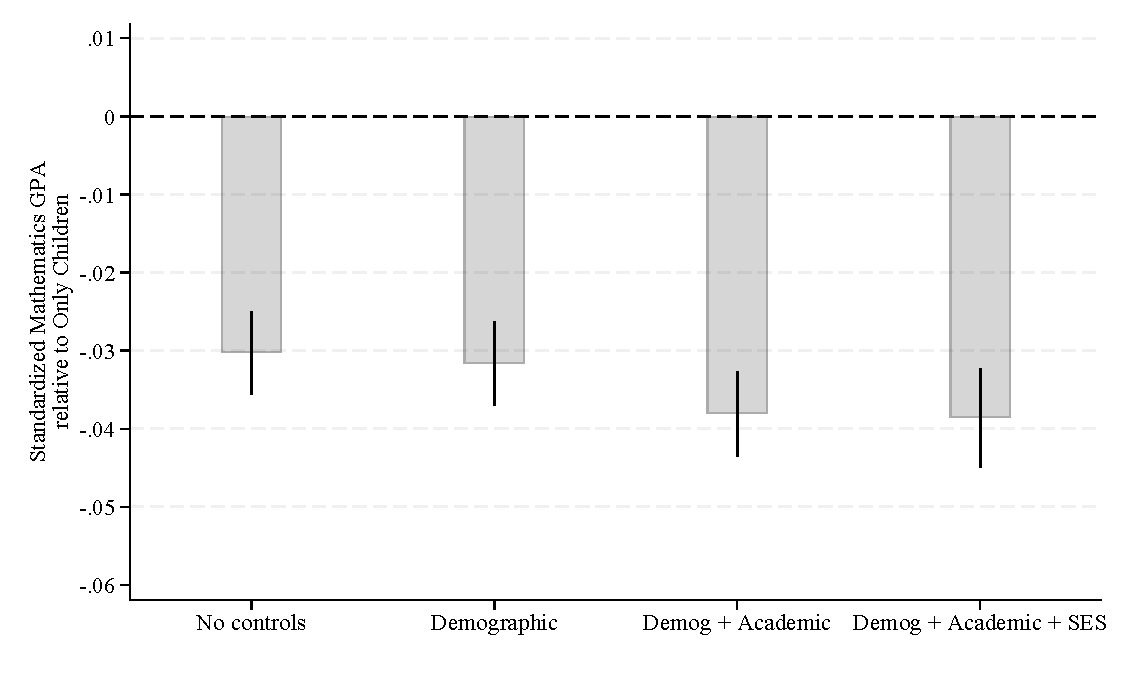
\includegraphics{./FIGURES/TWFE/twfe_std_gpa_m_adj_bycontrols_Tsiblings_Soldest_pairall_4.pdf}
      }
    }

      \begin{flushleft}
        \hyperlink{frame:twfe_gpa_controls_siblings}{\beamergotobutton{Results by siblings}}
        \hyperlink{frame:twfe_gpa_controls_1}{\beamergotobutton{6th-2nd grade}}
        \hyperlink{frame:twfe_gpa_controls_2}{\beamergotobutton{6th-4th grade}}
         \hyperlink{frame:twfe_gpa_controls_3}{\beamergotobutton{7th-4th grade}}
        \hyperlink{frame:twfe_gpa_controls_4}{\beamergotobutton{9th-8th grade}}  
    \end{flushleft}     
\end{frame}

\begin{frame}
    \label{frame:twfe_gpa_controls_siblings}
    \frametitle{And similar pattern when looking at effects by siblings}
        {\resizebox{0.9\textwidth}{!}{
        %\includegraphics{./FIGURES/TWFE/covid_twfe_C_bysibs_elm_all_gpa_m_adj_Tsiblings_Soldest_4.pdf}
       \includegraphics{./FIGURES/TWFE/twfe_std_gpa_m_adj_bycontrols_bysibs_Tsiblings_Soldest_pairall_4.pdf}
      }
    }

    \begin{flushleft}
        \hyperlink{frame:twfe_gpa_controls}{\beamergotobutton{Go Back $\carriagereturn$}}
    \end{flushleft}       

\end{frame}



\begin{frame}
    \label{frame:birthorder_intro}
    \frametitle{Similar results with first-born children}
        {\resizebox{0.9\textwidth}{!}{ \includegraphics{./FIGURES/Event Study/covid_event_bysibs_all_all_std_gpa_m_adj_Tsiblings_Soldest_4.pdf}
      }
    }  

    \begin{flushleft}
        \hyperlink{frame:mechanisms}{\beamergotobutton{Mechanisms}}
    \end{flushleft}
\end{frame}

% Show overlay 3 (Birth Order highlighted)
\againframe<3>{mechanisms}


\begin{frame}
    \label{frame:pcinternet}
    \frametitle{Similar effects with or without PC/Internet to fight for}
        {\resizebox{0.9\textwidth}{!}{
        %\includegraphics{./FIGURES/TWFE/covid_twfe_C_bysibs_elm_all_gpa_m_adj_Tsiblings_Soldest_4.pdf}
        \includegraphics{./FIGURES/TWFE/twfe_std_gpa_m_adj_bypc_int_Tsiblings_Soldest_pairall_4.pdf}
      }
    }

    \begin{flushleft}
        \hyperlink{frame:pcinternet_siblings}{\beamergotobutton{Results by siblings}}
    \end{flushleft}    

\end{frame}


% Show overlay 4 (Scarce material resources highlighted)  
\againframe<4>{mechanisms}


\begin{frame}
    \label{frame:siblingdisruption}
    \frametitle{Similar effects when siblings are 0-2 and 3-5 years apart}
        {\resizebox{0.9\textwidth}{!}{
        %\includegraphics{./FIGURES/TWFE/covid_twfe_C_bysibs_elm_all_gpa_m_adj_Tsiblings_Soldest_4.pdf}
        \includegraphics{./FIGURES/TWFE/twfe_gpa_age_gap_20_21_Tsiblings_Soldest_4.pdf}
      }
    }

    \begin{flushleft}
        \hyperlink{frame:siblingdisruption_siblings}{\beamergotobutton{Results by siblings}}
    \end{flushleft}    

\end{frame}



% Show overlay 5 (Sibling disruption highlighted)
\againframe<5>{mechanisms}

\begin{frame}
    \label{frame:parental_investments_vs_ses}
    \frametitle{Parental time helping with schoolwork is correlated with SES}
        {\resizebox{0.9\textwidth}{!}{
        \includegraphics{./FIGURES/Descriptive/parental_investment_ses.pdf}
      }
    }

\end{frame}


\begin{frame}
    \label{frame:byses}
    \frametitle{When parent's invest little time, there are smaller size effects}
        {\resizebox{0.9\textwidth}{!}{
        %\includegraphics{./FIGURES/TWFE/covid_twfe_C_bysibs_elm_all_gpa_m_adj_Tsiblings_Soldest_4.pdf}
        \includegraphics{./FIGURES/TWFE/twfe_std_gpa_m_adj_byses_Tsiblings_Soldest_pairall_4.pdf}
      }
    }

    \begin{flushleft}
        \hyperlink{frame:byses_siblings}{\beamergotobutton{Results by siblings}}
    \end{flushleft}    

\end{frame}

\begin{frame}
    \label{frame:byses_siblings}
    \frametitle{Similar pattern by number of siblings}
        {\resizebox{0.9\textwidth}{!}{
        %\includegraphics{./FIGURES/TWFE/covid_twfe_C_bysibs_elm_all_gpa_m_adj_Tsiblings_Soldest_4.pdf}
        \includegraphics{./FIGURES/TWFE/twfe_std_gpa_m_adj_byses_bysibs_Tsiblings_Soldest_pairall_4.pdf}
      }
    }

    \begin{flushleft}
        \hyperlink{frame:byses}{\beamergotobutton{Go Back $\carriagereturn$}}
    \end{flushleft}        

\end{frame}




\begin{comment}
\begin{frame}
    \label{frame:livesmother}
    \frametitle{Lives with mother}
        {\resizebox{0.9\textwidth}{!}{
        %\includegraphics{./FIGURES/TWFE/covid_twfe_C_bysibs_elm_all_gpa_m_adj_Tsiblings_Soldest_4.pdf}
        \includegraphics{./FIGURES/TWFE/twfe_gpa_lives_with_mother_20_21_Tsiblings_Soldest_4.pdf}
      }
    }

    \begin{flushleft}
        \hyperlink{frame:livesmother_siblings}{\beamergotobutton{Results by siblings}}
    \end{flushleft}    

\end{frame}

\begin{frame}
    \label{frame:livesmother_siblings}
    \frametitle{Lives with mother}
        {\resizebox{0.9\textwidth}{!}{
        %\includegraphics{./FIGURES/TWFE/covid_twfe_C_bysibs_elm_all_gpa_m_adj_Tsiblings_Soldest_4.pdf}
        \includegraphics{./FIGURES/TWFE/twfe_gpa_lives_with_mother_bysibs_20_21_Tsiblings_Soldest_4.pdf}
      }
    }

    \begin{flushleft}
        \hyperlink{frame:livesmother}{\beamergotobutton{Go Back $\carriagereturn$}}
    \end{flushleft}        

\end{frame}
\end{comment}




\begin{frame}
    \label{frame:childcare}
    \frametitle{But does having a child at home affect parents' investment in their siblings?}
       \begin{itemize}
            \item Children who turn 6 y.o after March 31st have to wait for the next school-year to enroll in 1st grade.
            \item That creates a cutoff. \\
                Born before $\rightarrow$ children go to school \\
                Born after $\rightarrow$  they stay at home.
            \item When schools are open, this creates a negative effect for siblings both in performance and parental time invested in them.
            \item This provides some evidence of the effect of having all children stay at home during school closures.
            \textcolor{green}{Think how to present these results...}
            %\item We use effects of delayed schooling (more childcare) outside of Covid to have a sense of how parents react to this.
            %\item Mixed results in literature (US and Denmark) although not until younger starts school.
        \end{itemize}
\end{frame}      

\begin{frame}
    \label{frame:delayedentry}
    \frametitle{Effects of delaying younger School Entry (GPA of older)}
    \input{./TABLES/rd_summ_1_m_a_365.tex}

      
    \only<2->{
    \highlightboxflex{-0.6}{-0.15}{1.2}{1.0}{draw=blue, draw opacity=0.8, dashed, fill=yellow!30, fill opacity=0.3}
    
    % Highlight box for Covid same sex coefficient  
    \highlightboxflex{1.85}{-0.15}{1.2}{1.0}{draw=blue, draw opacity=0.8, dashed, fill=yellow!30, fill opacity=0.3}
    
    \begin{tikzpicture}[overlay, remember picture]
        % Single text label at the bottom
        \node[red, above] at ([shift={(0,-2.8)}]current page.center) {\small Negative spillover of having a younger sibling stay at home};
        
        % Arrow to Pre-Covid coefficient (pointing to the left box)
        \draw[->, thick, blue, opacity=0.4] ([shift={(0,-2.2)}]current page.center) -- ([shift={(-0.6,-0.2)}]current page.center);
        
        % Arrow to Covid coefficient (pointing to the right box)
        \draw[->, thick, blue, opacity=0.4] ([shift={(0,-2.2)}]current page.center) -- ([shift={(1.85,-0.2)}]current page.center);
    \end{tikzpicture}
    }
\end{frame}

\begin{frame}
    \label{frame:delayedentryscores}
    \frametitle{Effects of delaying younger School Entry (Scores and investment)}
\makeatletter
     \centering
       \resizebox{0.95\textwidth}{!}%
{
\makeatother
\begin{tabular}{lccccc}
\toprule
& \multicolumn{2}{c}{Pre-Covid}  & \multicolumn{3}{c}{Post-Covid} \\
& \multicolumn{2}{c}{2018-2019}  & \multicolumn{3}{c}{2022-2024}  \\
\cmidrule(lr){2-3} \cmidrule(lr){4-6}
& Mathematics & Reading & Mathematics & Reading & Parental Time Investment  \\
& (1) & (2) & (3) & (4) & (5) \\
\bottomrule
&  &  &  & &  \\
\multirow{2}{*}{\shortstack[l]{Younger sibling born after \\ school-entry cutoff}}&      -0.025*  &      -0.023*  &      -0.009   &      -0.012   &      -0.035***\\
                    &     (0.014)   &     (0.012)   &     (0.013)   &     (0.010)   &     (0.013)   \\
Local Linear        &         Yes   &         Yes   &         Yes   &         Yes   &         Yes   \\
                    &               &               &               &               &               \\
Observations        &      86,605   &      86,602   &     104,983   &     105,064   &     101,766   \\
Counterfactual mean &      -0.105   &      -0.083   &       0.194   &       0.288   &      -0.004   \\
Bandwidth           &         365   &         365   &         365   &         365   &         365   \\
 

\bottomrule
\end{tabular}
}

    \only<2->{

    % Highlight box for Covid same sex coefficient  
    \highlightboxflex{3.20}{-0.60}{1.2}{1.0}{draw=blue, draw opacity=0.8, dashed, fill=yellow!30, fill opacity=0.3}
    
    \begin{tikzpicture}[overlay, remember picture]
        % Single text label at the bottom
        \node[red, above] at ([shift={(0,-2.8)}]current page.center) {\small Reduces parental time investment when younger sibling stays at home};

  
        
        % Arrow to Covid coefficient (pointing to the right box)
        \draw[->, thick, blue, opacity=0.4] ([shift={(0,-2.2)}]current page.center) -- ([shift={(3.20,-0.60)}]current page.center);
    \end{tikzpicture}
    }

\end{frame}



% Show overlay 6 (Parental dilution highlighted)
\againframe<6>{mechanisms}


\begin{frame}
    \label{frame:incomeshocks}
    \frametitle{No evidence of negative income shocks}
     
    %\input{./TABLES/MANUAL/twfe_ece_ses.tex}

     {\resizebox{0.9\textwidth}{!}{
        \includegraphics{./FIGURES/TWFE/twfe_ses_2_4_8_Tsiblings_Soldest_4.pdf}
      }
    }

    \begin{flushleft}
        \hyperlink{frame:incomeshocks_siblings}{\beamergotobutton{Results by siblings}}
    \end{flushleft}  

   
\end{frame}




\begin{frame}[t]
    \label{frame:iv_results}
    \frametitle{Same sex IV shows a reduction in family size effect during closures}
    \begin{table}[h]
\centering
\caption{Effect of Family Size on GPA}
\label{tab:twfe_twins}
\resizebox{0.95\textwidth}{!}{%
\begin{tabular}{lcccccc}
\hline
& \multicolumn{3}{c}{Pre-Covid} & \multicolumn{3}{c}{Covid} \\
\cmidrule(lr){2-4} \cmidrule(lr){5-7}
& First Stage & Second Stage & N & First Stage & Second Stage & N \\
\hline
\textbf{Instrument: twin at second birth} & 0.805*** & & 2,462,619 & 0.867*** & & 1,930,246 \\
(Sample: First child in families with two or more & (0.005) & & & (0.004) & & \\
births) & & & & & & \\
Number of children in family & & 0.007 & & & 0.012 & \\
& & (0.010) & & & (0.010) & \\
\textbf{Instrument: twin at third birth} & 0.813*** & & 1,861,964 & 0.874*** & & 1,272,826 \\
(Sample: first and second children in families & (0.005) & & & (0.005) & & \\
with three or more births) & & & & & & \\
Number of children in family & & $-0.009$ & & & $-0.010$ & \\
& & (0.010) & & & (0.012) & \\
\hline
\end{tabular}%
}
\end{table}
   
    \only<2->{
    \highlightboxflex{0.3}{-0.25}{0.8}{0.7}{draw=blue, draw opacity=0.8, dashed, fill=yellow!30, fill opacity=0.3}
    
    % Highlight box for Covid same sex coefficient  
    \highlightboxflex{3.55}{-0.25}{0.8}{0.7}{draw=blue, draw opacity=0.8, dashed, fill=yellow!30, fill opacity=0.3}
    
    \begin{tikzpicture}[overlay, remember picture]
        % Single text label at the bottom
        \node[red, above] at ([shift={(0,-2.8)}]current page.center) {\small Reduction in family size effect!};
        
        % Arrow to Pre-Covid coefficient (pointing to the left box)
        \draw[->, thick, blue, opacity=0.4] ([shift={(0,-2.2)}]current page.center) -- ([shift={(0.3,-0.25)}]current page.center);
        
        % Arrow to Covid coefficient (pointing to the right box)
        \draw[->, thick, blue, opacity=0.4] ([shift={(0,-2.2)}]current page.center) -- ([shift={(3.55,-0.25)}]current page.center);
    \end{tikzpicture}
    }
\end{frame}

% ========================================
% BEYOND PERFORMANCE
% ========================================

    \begin{frame}
            \label{frame:expectations}
            \frametitle{Reduction in educational expectations}
      {\resizebox{0.9\textwidth}{!}{
        \includegraphics{./FIGURES/TWFE/twfe_expectation_bysibs_2_4_8_Tsiblings_Soldest_4.pdf}
      }
    }   %\input{./TABLES/MANUAL/twfe_ece_expectations.tex}
    \end{frame}


%%%%%%%%%%%%%%%%%%%%%%%%%%%%%%%%%%%%%%%%%%%%%%%%%%%%%
%%%%%%%%%%%%%%%%%%%%%%%%%%%%%%%%%%%%%%%%%%%%%%%%%%%%%




\begin{frame}
    \label{frame:gpa_trends_grades_elm}
    \frametitle{Trends in data}
               \includegraphics[width=\textwidth]{./FIGURES/Descriptive/raw_grades_elm_std_gpa_m_adj_Tsiblings_Sall_Size2_4.pdf}    
    \begin{flushleft}
        \hyperlink{frame:gpa_trends}{\beamergotobutton{Go Back $\carriagereturn$}}
    \end{flushleft}   
    
    
\end{frame}

\begin{frame}
    \label{frame:gpa_trends_grades_sec}
    \frametitle{Trends in data}
               \includegraphics[width=\textwidth]{./FIGURES/Descriptive/raw_grades_sec_std_gpa_m_adj_Tsiblings_Sall_Size2_4.pdf}    
          \hyperlink{frame:gpa_trends}{\beamergotobutton{Go Back $\carriagereturn$}}
  
\end{frame}




\end{document}